\documentclass[runningheads]{llncs}

\usepackage[T1]{fontenc}
\usepackage[utf8]{inputenc}
\usepackage{amsmath,amssymb,amsfonts}
\usepackage{graphicx}
\usepackage{booktabs}
\usepackage{tabularx}
\usepackage{multirow}
\usepackage{array}
\usepackage{enumitem}
\usepackage{xcolor}
\usepackage{tikz}
\usetikzlibrary{arrows.meta,positioning,fit,calc,shapes.geometric}
\usepackage{placeins}
\usepackage{float}
\usepackage{threeparttable}
\usepackage{hyperref}
% Compatibility for the unchanged numeric citation calls in main3.
\makeatletter
\newcommand{\citep}[1]{%
  \begingroup
  \edef\ccis@citekeys{\zap@space#1 \@empty}%
  \expandafter\cite\expandafter{\ccis@citekeys}%
  \endgroup
}
\makeatother
% Allow line breaking without changing wording, margins, or font sizes.
\emergencystretch=2em

\definecolor{navy}{HTML}{17365D}
\definecolor{blue}{HTML}{2F75B5}
\definecolor{lightblue}{HTML}{EAF2F8}
\definecolor{green}{HTML}{548235}
\definecolor{lightgreen}{HTML}{EAF4E3}
\definecolor{orange}{HTML}{C55A11}
\definecolor{lightorange}{HTML}{FCE4D6}
\definecolor{reviewred}{HTML}{9C0006}
\definecolor{reviewfill}{HTML}{FFC7CE}


\hypersetup{
  colorlinks=true,
  linkcolor=navy,
  citecolor=navy,
  urlcolor=blue,
  pdfauthor={Anonymous Authors},
  pdftitle={A Replicable Theory-Guided LLM Workflow for Measuring Legal Delegation and Administrative Discretion}
}
\setlist{nosep,leftmargin=*}
\renewcommand{\arraystretch}{1.0}
\setlength{\textfloatsep}{8pt plus 1pt minus 2pt}
\setlength{\floatsep}{6pt plus 1pt minus 1pt}
\setlength{\intextsep}{6pt plus 1pt minus 1pt}
\newcommand{\systemname}{an anonymized research prototype}
\newcommand{\future}[1]{\textit{#1}}

\title{A Replicable Theory-Guided LLM Workflow for Measuring Legal Delegation and Administrative Discretion}

% \author{
% \IEEEauthorblockN{Anonymous Author(s)}
% \IEEEauthorblockA{\small Anonymous Institution\\
% Anonymous Location \\
% anonymous@example.com}
% }

\titlerunning{A Replicable Theory-Guided LLM Workflow}
\author{Anonymous Authors}
\authorrunning{Anonymous Authors}
\institute{}

\begin{document}
\maketitle
\vspace{-0.7 cm}

\begin{abstract}

Coding complex legal texts for nuanced institutional concepts is difficult to scale, replicate, and audit. Large language models can reduce the cost of coding and text analysis. However, one-shot classifications often obscure the judgments underlying the final result and are difficult to reproduce across models and runs. We develop a replicable, theory-guided LLM workflow that converts expert coding rules into a versioned, auditable measurement instrument. The workflow decomposes complex legal concepts into ordered judgments. It preserves prompts, settings, evidence, and intermediate outputs while distinguishing generative classifications from predefined coding rules. We demonstrate the approach by measuring legislative delegation and administrative discretion in U.S. financial-regulation laws. The workflow first predicts whether a law delegates authority. It then classifies the amount of authority and the strength of statutory constraints before assigning a five-category ordinal discretion rank. We implement the workflow in a research prototype that displays prompts, settings, outputs, validation rules, and execution records. We evaluate binary delegation classification and three rank-classification strategies across multiple language models on the 169-law expert-coded benchmark. Delegation classification performs well despite severe class imbalance, while more modest discretion-rank agreement across model-strategy combinations highlights the value of an auditable, theory-guided workflow.


\keywords{legal natural language processing \and large language models \and legislative delegation \and administrative discretion \and reproducible workflows \and quantitative legal coding}
\end{abstract}



\vspace{-0.2 cm}
\section{Introduction}
\vspace{-0.2 cm}

Political-economy theories of institutions specify how legal rules allocate authority and constrain its exercise. Empirical testing of these theories requires converting complex legal texts into structured measures of authority, constraint, and institutional design \cite{grimmer2013text}. Manually coding laws is difficult because institutional concepts are latent, multidimensional, and span multiple statutory provisions. This process requires expert coding rules, structured judgments, and the preservation of evidence supporting each decision. Administrative discretion is a useful example because it depends on both the authority delegated by the legislature and the constraints governing its use \cite{epstein1999delegating}.

Large language models (LLM) offer a scalable approach to legal coding. However, one-shot classification collapses linked judgments into a single output. A model may assign the correct rank for the wrong reason, produce a rank inconsistent with its stated assessment of delegation or constraints, or make errors that cannot be traced to a specific coding decision. Single-prompt approaches are therefore difficult to audit, revise, and reproduce across models and runs. A replicable measurement system must instead decompose the construct into ordered judgments, preserve the evidence and intermediate outputs, and apply the coding rules consistently.

We address this shortcoming by developing a theory-guided workflow that turns the measurement model into an executable sequence of decisions. First, the workflow determines whether a law delegates qualifying authority. If it does, the system separately classifies the amount of authority and the strength of statutory constraints, then combines those judgments to assign a discretion rank. We implement the workflow in \systemname{} to execute and record prompts, settings, intermediate outputs, and validation rules within a versioned, auditable framework. This paper makes four principal contributions:
\begin{enumerate}[nosep,leftmargin=*]
    \item \textbf{Replicable measurement instrument.} We develop an LLM-based instrument for measuring legal delegation and administrative discretion. The complete workflow, rather than an isolated prompt, is archived, versioned, and auditable.
    \item \textbf{Theory-guided workflow.} We translate an established formal model of delegation and discretion into an executable measurement workflow. The model identifies the concepts and relationships that define the variables used in empirical tests.
    \item \textbf{Transparent validation.} We separate generative LLM judgments from deterministic theoretical mappings and preserve the intermediate evidence needed to diagnose disagreements.
    \item \textbf{Research-facing prototype.} We enable domain researchers to apply and inspect the measurement process without directly managing prompts, APIs, model orchestration, or structured-output parsing.
\end{enumerate}

\noindent The objective is not to establish an autonomous legal coder. Rather, we show how expert-defined measurement can be made scalable, inspectable, and auditable.
\vspace{-0.2 cm}
\section{Measurement Task and Design Requirements}
\vspace{-0.1 cm}
\subsection{Delegation, Constraints, and Discretion}


Delegation is the transfer of policymaking authority from a legislature to an executive or administrative actor, enabling the agent to modify policy or regulate conduct. Legislatures may also impose substantive or procedural constraints that restrict the agent's ability to set policy, including administrative standards, approval requirements, deadlines, reporting obligations, and oversight reviews. Delegation alone, therefore, does not determine administrative discretion.

In principal-agent models of institutional design, administrative discretion is the agent's residual policy latitude after accounting for delegated authority and the constraints on its use \cite{epstein1999delegating,epstein1994administrative}. We operationalize this construct as
\begin{equation}
\mathrm{Discretion}=D(1-C),
\label{eq:discretion}
\end{equation}
where $D$ represents delegated authority and $C$ is the constraint index \cite{epstein1999delegating,ohalloran2015banking}. The workflow must therefore preserve the model's conceptual ordering: delegation is logically prior to discretion, and discretion depends on the authority transferred and the strength of the constraints governing that authority.

This measurement strategy builds on cumulative research on legislative delegation. Early formal models framed discretion as policy latitude that balances agency expertise against bureaucratic drift \citep{epstein1994administrative}, empirical studies combined delegated authority and statutory constraints into quantitative indices for U.S. financial laws \citep{ohalloran2015banking,ohalloran2016datascience,groll2021delegation}, and later work explored algorithmic extraction from legal text \citep{ohalloran2015markets}.

Expert coders applied these concepts by annotating legislative summaries. They measured delegated authority and statutory constraints as continuous components, then combined them to construct the discretion index in Eq.~\ref{eq:discretion}. Individually, they assigned each law to one of five ordinal discretion categories, 0--4, based on the total discretionary authority delegated and the restrictions on its exercise. The ordinal classification provides the expert-coded benchmark for the prediction task.


\vspace{-0.2 cm}
\subsection{Ordinal Operationalization}
The five-category ordinal benchmark was coded separately from the continuous discretion index. Rank 0 denotes no delegation. Conditional on delegation, Ranks 1--4 correspond to the four combinations of delegated authority (low or high) and statutory constraints (strong or weak). The ordinal benchmark, therefore, provides a separate expert-coded classification of total discretionary authority.

Let $x_i$ denote the legislative summary text for law $i$. The law is the unit of analysis. The measurement model contains three component variables: $d_i \in \{0,1\}$ indicates whether a law delegates policymaking authority, $a_i \in \{\mathrm{Low},\mathrm{High}\}$ denotes the amount of delegated authority, and $c_i \in \{\mathrm{Strong},\mathrm{Weak}\}$ denotes the strength of statutory constraints. For the prediction workflow, the discretion rank is $y_i^{\mathrm{map}}=m(d_i,a_i,c_i)$, where

\begin{equation}
 m(d_i,a_i,c_i)=
\begin{cases}
0, & d_i=0,\\
1, & d_i=1,\ a_i=\mathrm{Low},\ c_i=\mathrm{Strong},\\
2, & d_i=1,\ a_i=\mathrm{Low},\ c_i=\mathrm{Weak},\\
3, & d_i=1,\ a_i=\mathrm{High},\ c_i=\mathrm{Strong},\\
4, & d_i=1,\ a_i=\mathrm{High},\ c_i=\mathrm{Weak}.
\end{cases}
\label{eq:rankmap}
\end{equation}

The mapping encodes the theoretical relationship among delegation, authority, and constraints. It is part of the measurement model, not a learned relationship, and reflects the expert protocol's lexicographic ordering of the authority-constraint space. For example, high delegated authority with strong constraints is ranked above low delegated authority with weak constraints because the protocol gives primary weight to the scope of delegated jurisdiction. Ordinal evaluation therefore assesses whether the workflow reproduces the expert-coded 0--4 discretion benchmark, not whether it estimates the continuous index in Eq.~\ref{eq:discretion}.

\subsection{Computational Requirements}

LLMs have shown promise as low-cost annotators across text-annotation and qualitative tasks \citep{gilardi2023chatgpt,dai2023llm}. Those results do not establish reliability for nuanced legal constructs. Prompted generative models may perform poorly when applying domain-expert codebooks to specialized historical legal texts \citep{thalken2023modeling}. Legal NLP benchmarks such as LexGLUE and LegalBench likewise emphasize task-specific evaluation and expert-designed categories \citep{chalkidis2022lexglue,guha2023legalbench}. These findings motivate a conservative design in which LLM coding is evaluated against a controlled expert-coded benchmark and remains subject to expert review.

The workflow uses versioned LLM stages to estimate the component variables: $\hat d_i=g_D(x_i)$, $\hat a_i=g_A(x_i,\hat d_i)$, and $\hat c_i=g_C(x_i,\hat d_i,\hat a_i)$. The component stages also return structured evidence and rationales, collectively denoted by $r_i$. The prompts, inputs, outputs, rationales, evidence, and model settings are retained in the execution trace.

The system then applies one of three rank-classification strategies: Sequential Ordinal Cascade, Direct Multiclass Rank Prediction, and Two-Band Rank Classification. For strategy $s$, $\tilde y_i^{(s)}=h_s(x_i,\hat d_i,\hat a_i,\hat c_i,r_i)$. The theoretical mapping and the rank-classification strategies serve different functions. The mapping $m(\cdot)$ defines the construct, whereas $h_s(\cdot)$ estimates the final rank under alternative computational strategies.

For each law, the system computes the theory-implied rank $y_i^{\mathrm{map}}=m(\hat d_i,\hat a_i,\hat c_i)$ and compares it with the strategy-specific prediction $\tilde y_i^{(s)}$. Define the consistency indicator
\begin{equation}
q_i^{(s)} = \mathbf{1}\left[\tilde y_i^{(s)} = y_i^{\mathrm{map}}\right].
\label{eq:consistency}
\end{equation}
A value of $q_i^{(s)}=1$ indicates that the rank predicted by strategy $s$ agrees with the rank implied by the model's own delegation, authority, and constraint classifications. A disagreement is retained and flagged for review rather than silently overwritten. This design allows the evaluation to distinguish benchmark agreement from internal theoretical consistency.

The workflow also draws on weak supervision and interactive human-feedback systems \citep{ratner2017snorkel,cormack2014evaluation}, as well as prompt-chaining systems that decompose LLM tasks into modular, controllable steps \citep{wu2022aichains,wu2022promptchainer}. We do not claim to introduce human-in-the-loop annotation or prompt chaining. Rather, we integrate these computational approaches with a substantive political-economy measurement model so that expert coding rules determine the variables, dependencies, deterministic mappings, and validation checks used by the workflow. 
\vspace{-0.2 cm}
\section{Theory-Guided Workflow Architecture}
\vspace{-0.2 cm}
The system was developed iteratively to align LLM judgments with expert coding rules. The crucial methodological shift was from treating a single prompt as the coding instrument to treating the structured, multi-stage workflow graph as the instrument.

\subsection{From Expert Coding Rules to Workflow Logic}

We use the term \emph{theory-guided AI} to describe a computational design in which substantive theory structures the inference process. Delegation is logically prior to discretion. The workflow first predicts whether the law delegates authority, \(\hat d_i \in \{0,1\}\). If \(\hat d_i=0\), it assigns Rank 0 deterministically and skips the component-classification and rank-prediction stages. If \(\hat d_i=1\), the workflow identifies the relevant administrative actors, classifies the amount of delegated authority, \(\hat a_i \in \{\mathrm{Low},\mathrm{High}\}\), and the strength of statutory constraints, \(\hat c_i \in \{\mathrm{Strong},\mathrm{Weak}\}\), and retains the supporting evidence and rationale, \(r_i\). It then computes the component-implied rank, \(y_i^{\mathrm{map}}=m(\hat d_i,\hat a_i,\hat c_i)\), while the selected rank-classification strategy produces a separate prediction, \(\tilde y_i^{(s)}\). The workflow compares the two ranks using the consistency indicator \(q_i^{(s)}\) and stores the component values, strategy-specific prediction, evidence, model settings, and execution trace. Figure~\ref{fig:conceptual} summarizes this theory-guided sequence.

\begin{figure}[t]
\centering
\resizebox{0.88\textwidth}{!}{%
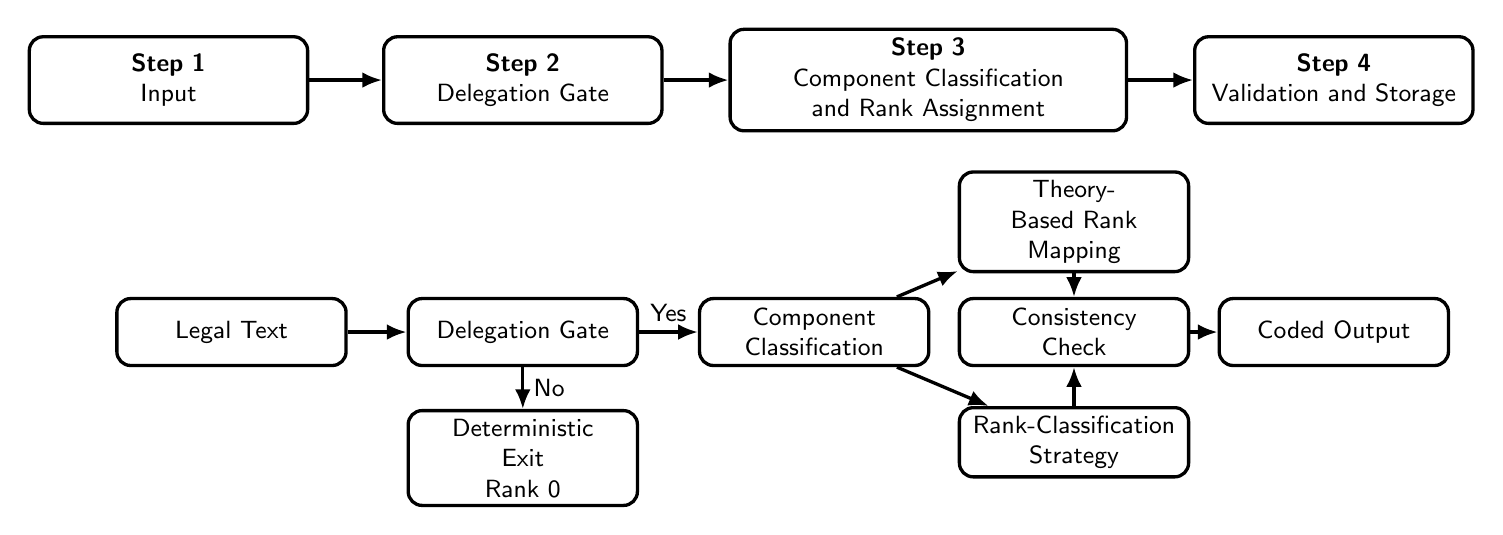
\begin{tikzpicture}[
  font=\sffamily\small,
  box1/.style={draw=black, rounded corners=5pt, very thick, align=center, fill=white, minimum height=1.1cm, text width=3.3cm},
  box1long/.style={draw=black, rounded corners=5pt, very thick, align=center, fill=white, minimum height=1.1cm, text width=4.8cm},
  box2/.style={draw=black, rounded corners=5pt, very thick, align=center, fill=white, minimum height=0.85cm, text width=2.7cm, inner sep=3pt},
  arrow/.style={-{Latex[length=2.5mm, width=2.0mm]}, very thick, draw=black}
]

% --- Row 1 ---
\node[box1] (s1) at (0, 3.2) {\textbf{Step 1}\\Input};
\node[box1] (s2) at (4.5, 3.2) {\textbf{Step 2}\\Delegation Gate};
\node[box1long] (s3) at (9.65, 3.2) {\textbf{Step 3}\\Component Classification\\and Rank Assignment};
\node[box1] (s4) at (14.8, 3.2) {\textbf{Step 4}\\Validation and Storage};

\draw[arrow] (s1) -- (s2);
\draw[arrow] (s2) -- (s3);
\draw[arrow] (s3) -- (s4);

% --- Row 2 ---
\node[box2] (legal) at (0.8, 0) {Legal Text};
\node[box2] (gate2) at (4.5, 0) {Delegation Gate};
\node[box2] (comp) at (8.2, 0) {Component\\Classification};

\node[box2] (exit) at (4.5, -1.6) {Deterministic\\Exit\\Rank 0};

\node[box2] (theory) at (11.5, 1.4) {Theory-\\Based Rank\\Mapping};
\node[box2] (check) at (11.5, 0) {Consistency\\Check};
\node[box2] (strat) at (11.5, -1.4) {Rank-Classification\\Strategy};

\node[box2] (coded) at (14.8, 0) {Coded Output};

% --- Arrows Row 2 ---
\draw[arrow] (legal) -- (gate2);
\draw[arrow] (gate2) -- node[above, font=\sffamily\small] {Yes} (comp);
\draw[arrow] (gate2) -- node[right, font=\sffamily\small] {No} (exit);

\draw[arrow] (comp) -- (theory);
\draw[arrow] (comp) -- (strat);
\draw[arrow] (theory) -- (check);
\draw[arrow] (strat) -- (check);
\draw[arrow] (check) -- (coded);

\end{tikzpicture}%
}

\caption{Four-stage theory-guided classification workflow.}
\label{fig:conceptual}
\end{figure}

This dependency structure addresses a recurrent failure of independent-column coding: a later variable, such as \texttt{discretion\_rank}, cannot reliably use an earlier delegation decision unless the pipeline stores and forwards that decision. In the prototype, the system determines execution order by topologically sorting the directed acyclic graph, preventing stale forward references that arise when visual column order is treated as execution order. Each node records inputs, outputs, status, timing, and, where applicable, evidence and rationale.


\vspace{-0.2 cm}

\subsection{Executable Workflow Operations}

Table~\ref{tab:algorithm} translates the measurement logic into the executable sequence implemented by the workflow. It distinguishes LLM-assisted judgments from deterministic operations and shows how the system moves from source-text ingestion through delegation screening, component classification, rank prediction, consistency validation, and output storage.

\begin{table}[t]
\caption{Algorithmic execution of the theory-guided discretion workflow.}
\label{tab:algorithm}
\centering
\footnotesize
\begin{tabular}{@{}>{\raggedright\arraybackslash}p{0.06\columnwidth}>{\raggedright\arraybackslash}p{\dimexpr0.94\columnwidth-2\tabcolsep\relax}@{}}
\hline
\textbf{Step} & \textbf{Operation and Logic} \\
\hline

1 &
\textbf{Load Source Text:}
Read source text \(x_i\) and attach
stable identifiers. \\

2 &
\textbf{Delegation Gate (LLM):}
Estimate
\(\hat d_i=g_D(x_i)\in\{0,1\}\)
and retain the supporting evidence and rationale. \\

3 &
\textbf{Early Exit (Deterministic):}
If \(\hat d_i=0\), set the theory-implied rank
\(y_i^{\mathrm{map}}=0\), assign the required default values, and stop
the delegated-discretion branch. \\

4 &
\textbf{Component Classification (LLM):}
Conditional on \(\hat d_i=1\), identify the relevant administrative
actors, classify delegated authority
\(\hat a_i\in\{\mathrm{Low},\mathrm{High}\}\), classify statutory
constraints
\(\hat c_i\in\{\mathrm{Strong},\mathrm{Weak}\}\), and retain the
supporting evidence and rationales \(r_i\). \\

5 &
\textbf{Strategy-Specific Rank Prediction (LLM):}
Apply the selected rank-classification strategy. The Sequential
Ordinal Cascade uses
successive early-exit binary decisions; Direct Multiclass predicts
Ranks \(1\)--\(4\) in one step; and Two-Band first predicts a
lower/higher rank band and then classifies within the selected band. \\

6 &
\textbf{Theoretical Consistency Validation (Deterministic):}
Compute
\(y_i^{\mathrm{map}}=m(\hat d_i,\hat a_i,\hat c_i)\)
and compare it with the strategy-specific prediction
\(\tilde y_i^{(s)}\). Record the consistency indicator
\(q_i^{(s)}\) and flag any disagreement. \\

7 &
\textbf{Output Serialization:}
Store the component classifications, theory-implied rank,
strategy-specific rank, consistency flag, evidence, prompts, model
settings, execution trace, runtimes, token use, cost, and final
reported output. \\

\hline
\end{tabular}
\end{table}

 The engine implements the workflow through document-input, LLM, conditional-routing, deterministic-value, validation, and output nodes. The workflow retains both the strategy-specific prediction \(\tilde y_i^{(s)}\) and the theory-implied rank \(y_i^{\mathrm{map}}\). Strategy-specific predictions are used for comparative evaluation and are not silently replaced when they conflict with the deterministic component mapping. Instead, the validation node records the disagreement with an inconsistency flag. This separation allows researchers to evaluate agreement with the expert-coded benchmark separately from the workflow's internal consistency in linking delegation, authority, constraints, and discretion.

 A one-shot prediction collapses the relationships among delegation, authority, constraints, and discretion into an opaque judgment. The workflow makes the measurement assumptions inspectable and testable. Researchers can locate a disagreement at the Delegation Gate, authority classification, constraint classification, rank-classification strategy, or consistency check. 

Figure~\ref{fig:reproducibility} illustrates the reproducibility architecture. The system archives the source corpus, the workflow JSON schema and definition hash (SHA-256), model configurations, and a comprehensive node-level execution trace to ensure that any coded dataset can be audited and reconstructed. The prototype implements the workflow as an auditable research instrument, not as a production system.


\begin{figure}[t]
\centering
\resizebox{0.78\textwidth}{!}{\input{figures/reproducibility_flow.tex}}
\caption{Reproducibility and execution tracking pipeline.}
\label{fig:reproducibility}
\end{figure}
\vspace{-0.2 cm}
\subsection{Audit Record and Reproducibility}
\vspace{-0.2 cm}
Human expertise enters before, during, and after model execution. Before execution, domain experts define the construct, identify its constituent dimensions, delimit the source set, specify coding rules, and determine the relationships the workflow must preserve. During evaluation, experts distinguish extraction errors from conceptual boundary cases. After evaluation, they decide whether a disagreement warrants a local case correction, revision of an operational rule, or reconsideration of the historical benchmark.


\textbf{Method-level revision.} Researchers revise the codebook, source-selection rules, stage prompts, workflow dependencies, output definitions, and deterministic mappings. Because these changes alter the general measurement rule, they create a new workflow version to preserve comparability across model runs.
 
\textbf{Case-level adjudication.} For an individual coded law, a researcher can inspect final values and node-by-node execution traces through an interactive visual dashboard. The interface displays side-by-side supporting rationales ($r_i$), flags discrepancies where $\tilde y_i^{(s)} \ne y_i^{\mathrm{map}}$, and supports manual value overrides or LLM re-evaluation with corrective feedback. The audit history tracks these local overrides without altering the global codebook or prompts for other cases.



\vspace{-0.3 cm}
\section{Benchmark, Experimental Design, and Results}
\vspace{-0.3 cm}
\subsection{Benchmark and source discipline}

The benchmark consists of 169 U.S. financial-regulation laws coded under a consistent protocol using legislative summaries from 1950--2013. We use CQ legislative summaries because they provide the standardized source corpus used in the foundational political-economy studies of delegation and discretion \citep{epstein1999delegating,ohalloran2015banking}. Using the same source texts preserves comparability with the original coding and avoids introducing variation from full-statute length and structure. Of these laws, 161 delegated authority, and eight did not. Expert coders assigned 0--4 discretion labels directly from legislative summaries based on the total discretionary authority delegated and the restrictions on its exercise. We treat these labels as the benchmark for replication rather than as legal truth. Benchmark runs use the same summaries to preserve consistency with the original coding.

\vspace{-0.35 cm}
\subsection{Evaluation levels}
The empirical evaluation asks whether LLMs can reproduce a theory-based measurement instrument, rather than simply generate plausible descriptions of statutes. We evaluate the workflow at three levels: whether it identifies qualifying delegation, whether the final discretion rank agrees with the expert-coded benchmark, and whether the strategy-specific rank is internally consistent with the delegation, authority, and constraint judgments produced by the workflow.

We separate the evaluation into two prediction tasks:

\begin{enumerate}[nosep]

    \item \textbf{Delegation Stage}: Binary delegation classification is evaluated on the full benchmark ($N=169$).

    \item \textbf{Discretion Stage}: Ordinal rank classification ($1$--$4$) is evaluated for laws with expert-coded delegation, with completed sample sizes reported by model-strategy configuration.

\end{enumerate}

\vspace{-0.3 cm}
\subsection{Controlled prompt and workflow comparison}

To evaluate discretion ranking, we implement and compare three workflow-based rank-classification strategies against a one-shot baseline. Table~\ref{tab:strategies_comparison} summarizes these strategies.

\begin{table}[t]
\centering
\caption{Comparison of evaluation strategies.}
\label{tab:strategies_comparison}
\footnotesize
\begin{tabularx}{\textwidth}{@{}
>{\raggedright\arraybackslash}p{0.26\textwidth}
>{\raggedright\arraybackslash}p{0.10\textwidth}
>{\raggedright\arraybackslash}X
>{\raggedright\arraybackslash}p{0.13\textwidth}@{}}
\toprule
\textbf{Strategy} & \textbf{Inputs} & \textbf{Decision process} & \textbf{Output} \\
\midrule
One-shot baseline & Source text & Single LLM prediction with no intermediate guidance & Discretion Rank 0--4 \\
Sequential Ordinal Cascade & Stage outputs & Evaluates early-exit binary splits: Rank 0 vs. Ranks 1--4 (delegation gate), then Rank 1 vs. Ranks 2--4, then Rank 2 vs. Ranks 3--4, and Rank 3 vs. Rank 4 & Discretion Rank 0--4 \\
Direct Multiclass Rank Prediction & Stage outputs & Predicts 1--4 directly using extracted authority and constraints & Discretion Rank 0--4 \\
Two-Band Rank Classification & Stage outputs & Low-rank vs. high-rank band split, then within-band classification & Discretion Rank 0--4 \\

\bottomrule
\end{tabularx}
\end{table}
\vspace{-0.3 cm}

\subsection{Experimental protocol}

We use the following experimental protocol:
\begin{itemize}[nosep]
    \raggedright
    \item \textbf{Models}: We evaluate Gemini 3.5 (\texttt{gemini-3.5-flash-lite}), Qwen 3 (\texttt{qwen/qwen3-235b-a22b-2507}), DeepSeek (\texttt{deepseek/deepseek-chat}), Kimi K2.5 (\texttt{moonshotai/kimi-k2.5}), and GPT-OSS (\texttt{openai/gpt-oss-120b}). The unconstrained One-Shot Baseline is evaluated only on Gemini 3.5.
    
    \item \textbf{Settings}: We set temperature to 0.0 to reduce sampling variation and record exact model identifiers and execution timestamps.
    
    \item \textbf{Output Format}: Each node returns structured JSON validated against a Pydantic schema.
    
    \item \textbf{Retries and Failures}: If a model call fails, times out, or returns invalid structured output, the system retries it up to three times using the same prompt, parameters, and schema. Persistent failures are recorded in the execution log.
\end{itemize}


\vspace{-0.2cm}
\subsubsection{Metrics}

For the binary delegation task, we report accuracy, balanced accuracy, class-specific precision and recall, and macro-F1. For the ordinal discretion task, we report exact-match accuracy, within-one accuracy ($W_1$), mean absolute error, linear weighted kappa, and quadratic weighted kappa. Weighted kappa is sensitive to marginal class imbalance in smaller samples. We therefore use $W_1$ as the primary operational indicator for expert screening while also reporting exact match, error, and weighted-kappa measures.

\vspace{-0.3 cm}
\subsection{Results and Diagnostics}
\vspace{-0.2 cm}
\subsubsection{Binary delegation}

Table~\ref{tab:binary} reports binary delegation screening results on the full delegation benchmark ($N=169$). The benchmark is severely imbalanced: 161 laws delegated authority and eight did not. We compare the final Delegation Gate against an earlier broad-screening baseline (\emph{High-Recall Screen}). The High-Recall Screen relied on broad semantic matching for any grant of power. The Delegation Gate uses explicit exclusions for routine administrative housekeeping, technical statutory amendments, and advisory commissions lacking binding rulemaking or enforcement authority.


\begin{table}[htbp]
\centering
\caption{Binary delegation stage screening results ($N=169$).}
\label{tab:binary}
\small
\begin{tabular}{@{}l@{\hspace{3pt}}rr@{}}
\toprule
\textbf{Metric} & \textbf{High-Recall Screen} & \textbf{Delegation Gate} \\
\midrule
Overall Accuracy & 94.67\% & 91.72\% \\
Balanced Accuracy & 73.45\% & 89.71\% \\
Positive Recall (Delegation) & 96.89\% & 91.93\% \\
Negative Recall & 50.00\% & 87.50\% \\
Positive Precision & 97.50\% & 99.33\% \\
Negative Precision & 44.44\% & 35.00\% \\
Macro-F1 & 72.13\% & 72.74\% \\
\midrule
TP / FN / TN / FP & 156 / 5 / 4 / 4 & 148 / 13 / 7 / 1 \\
\bottomrule
\end{tabular}
\end{table}

A naive majority-class baseline predicting delegation for all cases achieves 95.27\% raw accuracy. Yet it yields only 50.00\% balanced accuracy and fails on non-delegation statutes (0.00\% negative recall). In contrast, the High-Recall Screen yields slightly higher raw accuracy due to class imbalance, while the conservative Delegation Gate detects seven of the eight rare negative cases (87.50\% negative recall), achieving 89.71\% balanced accuracy and 72.74\% macro-F1.
\vspace{-0.4cm}
\subsubsection{Diagnosing disagreement}

The law PL83-577 illustrates why source discipline and intermediate evidence matter. The benchmark codes it as non-delegation (Rank 0). An exploratory staged run instead identified Securities and Exchange Commission rulemaking and exemption authority and classified the law as delegating authority. This disagreement could reflect an overbroad coding rule, a difference in source policy, or a mismatch between historical summary coding and full statutory detail. The trace does not by itself determine which label is correct; it makes the source of the disagreement visible for expert adjudication.

\vspace{-0.5cm}
\subsubsection{Discretion rank and model comparison}
Table~\ref{tab:multimodel_large} reports the cross-model evaluation of the three ranking strategies alongside an unconstrained One-Shot baseline on the expert-coded delegated-law benchmark ($N=161$ total available delegated statutes, with completed sample sizes reported per configuration).

\begin{table}[t]
\centering
\begin{threeparttable}

\caption{Cross-model evaluation results across ranking strategies and unconstrained baseline.}
\label{tab:multimodel_large}
\scriptsize
\setlength{\tabcolsep}{2.5pt}

\begin{tabular}{@{}llrrrrrr@{}}
\toprule
\textbf{Model} & \textbf{Strategy} & \textbf{$N$} & \textbf{Exact} & \textbf{W1} & \textbf{MAE} & \textbf{Linear $\kappa_w$} & \textbf{Quad $\kappa_w$} \\
\midrule

\multirow{4}{*}{Gemini 3.5} 
  & One-Shot Baseline (Unconstrained) & 140 & 28.6\% & 62.1\% & 1.250 & 0.051 & 0.042 \\
  & Sequential Ordinal Cascade        & 117 & 29.9\% & 75.2\% & 1.077 & 0.104 & 0.094 \\
  & Direct Multiclass Prediction      & 117 & 41.9\% & 76.9\% & 0.915 & 0.207 & 0.157 \\
  & Two-Band Classification           & 117 & 29.9\% & 65.8\% & 1.188 & 0.044 & 0.010 \\
\midrule

\multirow{3}{*}{Qwen 3} 
  & Sequential Ordinal Cascade        & 129 & 25.6\% & 65.9\% & 1.225 & 0.062 & 0.059 \\
  & Direct Multiclass Prediction      & 129 & 32.6\% & 64.3\% & 1.171 & 0.105 & 0.093 \\
  & Two-Band Classification           & 129 & 17.8\% & 48.8\% & 1.620 & 0.030 & 0.010 \\
\midrule

\multirow{3}{*}{DeepSeek} 
  & Sequential Ordinal Cascade        & 129 & 20.9\% & 57.4\% & 1.434 & 0.022 & 0.010 \\
  & Direct Multiclass Prediction      & 129 & 29.5\% & 71.3\% & 1.140 & 0.055 & 0.014 \\
  & Two-Band Classification           & 129 & 8.5\%  & 41.9\% & 1.837 & -0.014 & -0.020 \\
\midrule

\multirow{3}{*}{Kimi K2.5} 
  & Sequential Ordinal Cascade        & 60 & 30.0\% & 63.3\% & 1.317 & 0.133 & 0.094 \\
  & Direct Multiclass Prediction      & 60 & 21.7\% & 60.0\% & 1.433 & 0.076 & 0.067 \\
  & Two-Band Classification           & 60 & 15.0\% & 45.0\% & 1.700 & -0.008 & -0.003 \\
\midrule

\multirow{3}{*}{GPT-OSS} 
  & Sequential Ordinal Cascade        & 85 & 20.0\% & 55.3\% & 1.482 & 0.056 & 0.067 \\
  & Direct Multiclass Prediction      & 85 & 32.9\% & 69.4\% & 1.129 & 0.106 & 0.072 \\
  & Two-Band Classification           & 85 & 9.4\%  & 37.6\% & 1.871 & 0.007 & 0.021 \\
\bottomrule
\end{tabular}

\begin{tablenotes}
\scriptsize
\vspace{3mm}
\item[] \textit{Note:} $N$ reports completed evaluations per configuration; varying sample sizes across rows reflect provider rate limits during evaluation runs. The unconstrained One-Shot Baseline is evaluated on Gemini 3.5.
\end{tablenotes}

\end{threeparttable}
\end{table}

For Gemini 3.5, Direct Multiclass Rank Prediction performs best: exact-match accuracy increases from 28.6\% for the One-Shot Baseline to 41.9\%, within-one accuracy rises from 62.1\% to 76.9\%, and mean absolute error falls from 1.250 to 0.915. The One-Shot Baseline is an illustrative Gemini comparison that shows workflow gains for that model, rather than a cross-model result.

Within-one accuracy exceeds exact-match accuracy across all configurations, reaching 76.9\% for Gemini 3.5 and 71.3\% for DeepSeek. This pattern shows that many errors are near misses rather than large ordinal departures. Because legal codebooks require nuanced boundary judgments on statutory constraints, adjacent agreement is useful for expert screening even when exact rank agreement remains limited. Rather than replacing human expertise, the workflow functions as a triage and auditing instrument: it screens non-delegation laws with high balanced accuracy (89.7\%) and surfaces supporting rationales, enabling scholars to audit boundary cases without recoding the full source corpus.

Table~\ref{tab:consistency} reports diagnostic consistency for 15 statutes ($N=15$): agreement between predicted discretion ranks and those implied by the workflow's delegation, authority, and constraint classifications ($q_i^{(s)} = \mathbf{1}[\tilde y_i^{(s)} = y_i^{\mathrm{map}}]$). Consistency ranges from 6.7\% to 73.3\%, highest for Gemini 3.5 Two-Band Rank Classification. The discrepancies flag internal disagreements for expert review.

\vspace{2mm}
\begin{table}[htbp]
\centering
\caption{Diagnostic internal theoretical consistency check ($N=15$, \%).}
\label{tab:consistency}
\scriptsize
\begin{tabular}{@{}lccc@{}}
\toprule
\textbf{Model} & \textbf{Cascade} & \textbf{Direct} & \textbf{Two-Band} \\
\midrule
Gemini 3.5 & 53.3 & 33.3 & 73.3 \\
Qwen 3     & 33.3 & 46.7 & 26.7 \\
DeepSeek   & 46.7 & 66.7 & 26.7 \\
Kimi K2.5  & 46.7 & 66.7 & 46.7 \\
GPT-OSS    & 6.7  & 46.7 & 6.7  \\
\bottomrule
\end{tabular}

\vspace{3mm}
\parbox{\columnwidth}{\scriptsize \textit{Note:} Evaluated on a diagnostic 15-statute test sample where component-level authority and constraint features were extracted in parallel with all three ranking strategies.}
\end{table}



\clearpage
\section{Discussion, Limitations, and Conclusion}
\vspace{-0.2cm}
\paragraph{Reproducibility.} Replication requires preserving the source set, stable law identifiers, workflow definition, prompts, typed outputs, model settings, execution trace, benchmark comparison, case-level adjudications, and exported dataset. Because the workflow, rather than a single prompt, is the measurement instrument, these materials must remain linked to the version used to produce each coded output.
\vspace{-0.2cm}
\paragraph{Limitations.} Three limitations remain. First, the evaluation relies on legislative summaries rather than full statutory text, preserving comparability with the expert benchmark while leaving full-text validation for future work. Second, the benchmark reflects U.S. financial regulation, preserving within-domain construct validity while leaving cross-domain external validity for subsequent studies. Third, LLM classifications remain sensitive to model choice, prompt wording, and provider updates.
\vspace{-0.2cm}

\paragraph{Future Work.} Future work will evaluate held-out laws, measure component-level authority and constraint accuracy, test additional policy domains, extend one-shot baselines across model backends, and use independent expert recoding to establish human intercoder reliability.
\vspace{-0.2cm}
\paragraph{Conclusions.} This paper addressed the challenge of recovering delegated authority and administrative discretion from legal text. Rather than relying on black-box classifiers or opaque prompts, we introduced a theory-guided LLM workflow where delegation, authority, and constraints are modeled as distinct, interdependent components with deterministic theoretical mapping. Human experts govern the rules, validation, and adjudication. The resulting system makes latent institutional measurement explicit, structured, inspectable, and reproducible.



\bibliographystyle{splncs04}
\vspace{-0.2cm}
\bibliography{references}
\vspace{-0.2cm}
\end{document}

